\documentclass[final]{beamer}
%% Possible paper sizes: a0, a0b, a1, a2, a3, a4.
%% Possible orientations: portrait, landscape
%% Font sizes can be changed using the scale option.
\usepackage[size=a0,orientation=portrait,scale=1.25]{beamerposter}
\usepackage{amsmath, amsthm}
\usetheme{gemini}
\usecolortheme{seagull}
\useinnertheme{rectangles}

\usepackage{caption}
\usepackage{subcaption}
% ====================
% Packages
% ====================

\usepackage[utf8]{vietnam}
\usepackage{graphicx}
\usepackage{booktabs}
\usepackage{tikz}
\usepackage{pgfplots}

% ====================
% Lengths
% ====================

% If you have N columns, choose \sepwidth and \colwidth such that
% (N+1)*\sepwidth + N*\colwidth = \paperwidth
\newlength{\sepwidth}
\newlength{\colwidth}
\setlength{\sepwidth}{0.01\paperwidth}
\setlength{\colwidth}{0.48\paperwidth}

\newcommand{\separatorcolumn}{\begin{column}{\sepwidth}\end{column}}

% ====================
% Logo (optional)
% ====================

% Thêm \hspace*{3cm} ở ĐẦU để đẩy logo trái sang phải
\logoleft{\hspace*{1cm}
\includegraphics[width=10cm, keepaspectratio]{logos/HCMUS.png}}

% Thêm \hspace*{3cm} ở CUỐI để đẩy logo phải sang trái
\logoright{
\includegraphics[width=10cm, keepaspectratio]{logos/VLHN.png}\hspace*{1cm}}
% ====================
% Footer (optional)
% ====================

\footercontent{
	Hội nghị Khoa học Trường Đại học Khoa học tự nhiên, ĐHQG-HCM lần thứ 15 năm 2026 \hfill
	\insertdate \hfill
	\href{mailto:huytranquoc298@gmail.com}{\texttt{huytranquoc298@gmail.com}}
}
% (can be left out to remove footer)
% ====================
% BibLaTeX
% ====================

\usepackage[backend=biber, style=ieee, sorting=none]{biblatex}

%% Dùng số [1], [2] thay vì icon tài liệu mặc định của Beamer trong danh mục tài liệu tham khảo
\setbeamertemplate{bibliography item}[text]

%% Reference Sources
\addbibresource{refs.bib}
\renewcommand{\pgfuseimage}[1]{\includegraphics[scale=1]{#1}}

\title{Xây dựng phần mềm PEAKFIT \\ trong việc phân tích phổ tia gamma }

\author{Trần Quốc Huy\inst{1} \and Châu Thành Tài \inst{1}$^{,*}$ \and Lê Anh Nhi \inst{1} \and Trần Thiện Thanh \inst{1}  \and Châu Văn Tạo \inst{1}}

\institute[shortinst]{\inst{1} Bộ môn Vật lý Hạt nhân – Kỹ thuật Hạt nhân – Vật lý Y khoa, Khoa Vật lý – Vật lý Kỹ thuật, Đại học Khoa học Tự nhiên, Đại học Quốc gia Thành phố Hồ Chí Minh, Việt Nam}

\date{January 01, 2025}

\begin{document}
	
\begin{frame}[t]
	
	\begin{columns}[t]
	
	\begin{column}{2\colwidth+\sepwidth}
	\begin{block}{Tóm tắt}
		Mục tiêu của nghiên cứu này là phát triển phần mềm PEAKFIT phục vụ đọc, xử lý và phân tích phổ gamma thông qua một giao diện đồ họa thân thiện với người dùng. 
		Phần mềm được phát triển bằng ngôn ngữ C\# và tích hợp thuật toán Mariscotti để tự động nhận diện các đỉnh phổ. 
		Các mô-đun hiệu chuẩn năng lượng, hiệu chuẩn độ rộng toàn phần tại nửa cực đại (FWHM) và hiệu chuẩn hiệu suất 
		cũng được tích hợp nhằm cung cấp một quy trình phân tích phổ thống nhất. PEAKFIT hỗ trợ trực quan hóa phổ, 
		xác định và hiệu chỉnh các đỉnh, thực hiện các phép khớp hiệu chuẩn và lưu trữ các tham số cần thiết cho quá trình 
		phân tích. Các thử nghiệm ban đầu cho thấy phần mềm có khả năng xử lý ổn định các phổ gamma thử nghiệm và thực hiện 
		các chức năng phân tích đã thiết kế. Kết quả cho thấy PEAKFIT có tiềm năng trở thành một công cụ thuận tiện và có 
		khả năng tiếp cận cao cho phân tích phổ gamma trong nghiên cứu và đào tạo hạt nhân.
		
	\end{block}
	\end{column}

	\end{columns}

	\begin{columns}[t]
		\separatorcolumn
		
		\begin{column}{\colwidth}
			
			% \begin{box}{Mục tiêu}
				
			% 	\begin{itemize}
			% 		\item Tự động phân tích đỉnh bằng cách phát triển các thuật toán tìm đỉnh : Mariscotti, Savitzky-Golay.
			% 		\item Tối ưu độ chính xác và ứng dụng.
			% 	\end{itemize}
				
			% 	Eget augue porta, bibendum venenatis tortor.
				
			% \end{box}
			\begin{block}{Giới thiệu}
				PEAKFIT là phần mềm có giao diện đồ họa, được phát triển bằng C\# để đọc, hiển thị và phân tích phổ gamma. 
				Phần mềm tích hợp chức năng tìm đỉnh tự động và các công cụ hiệu chuẩn năng lượng, hiệu suất và độ rộng đỉnh (FWHM).
			\end{block}

			\begin{block}{Các chức năng của PEAKFIT}
				
				\begin{enumerate}
					\item \textbf{Thuật toán nhận diện đỉnh :} \\
					PEAKFIT Sử dụng thuật toán Mariscotti với hàm sai phân bậc 2 $S_i$ và độ lệch chuẩn $F_i$ để tìm kiếm đỉnh. \\ 
					Xác định hàm sai phân bậc hai với hàm rời rạc : 
					\begin{equation}
						S_i =\sum_{j}C_{ij}(z, w) N_j \quad \text{\cite{mariscotti1967method}}
					\end{equation}
					Trong đó : $C_{ij}$ là hệ số trọng số. 
					và độ lệch chuẩn của hàm sai phân bậc hai : 
					\begin{equation}
						F_i = \left(\sum_{j}C_{ij}^2(z, w) N_j\right)^{1/2} \quad \text{\cite{mariscotti1967method}}
					\end{equation}
					Đánh giá đỉnh dựa trên 4 điều kiện ràng buộc: biên độ đỉnh ($|S_{i_1}| > f \cdot F_{i_1}$), độ rộng đỉnh $w$, và các tham số dung sai $\epsilon$, hệ số tin cậy $f$\\
					\begin{figure}[t]
						\centering
						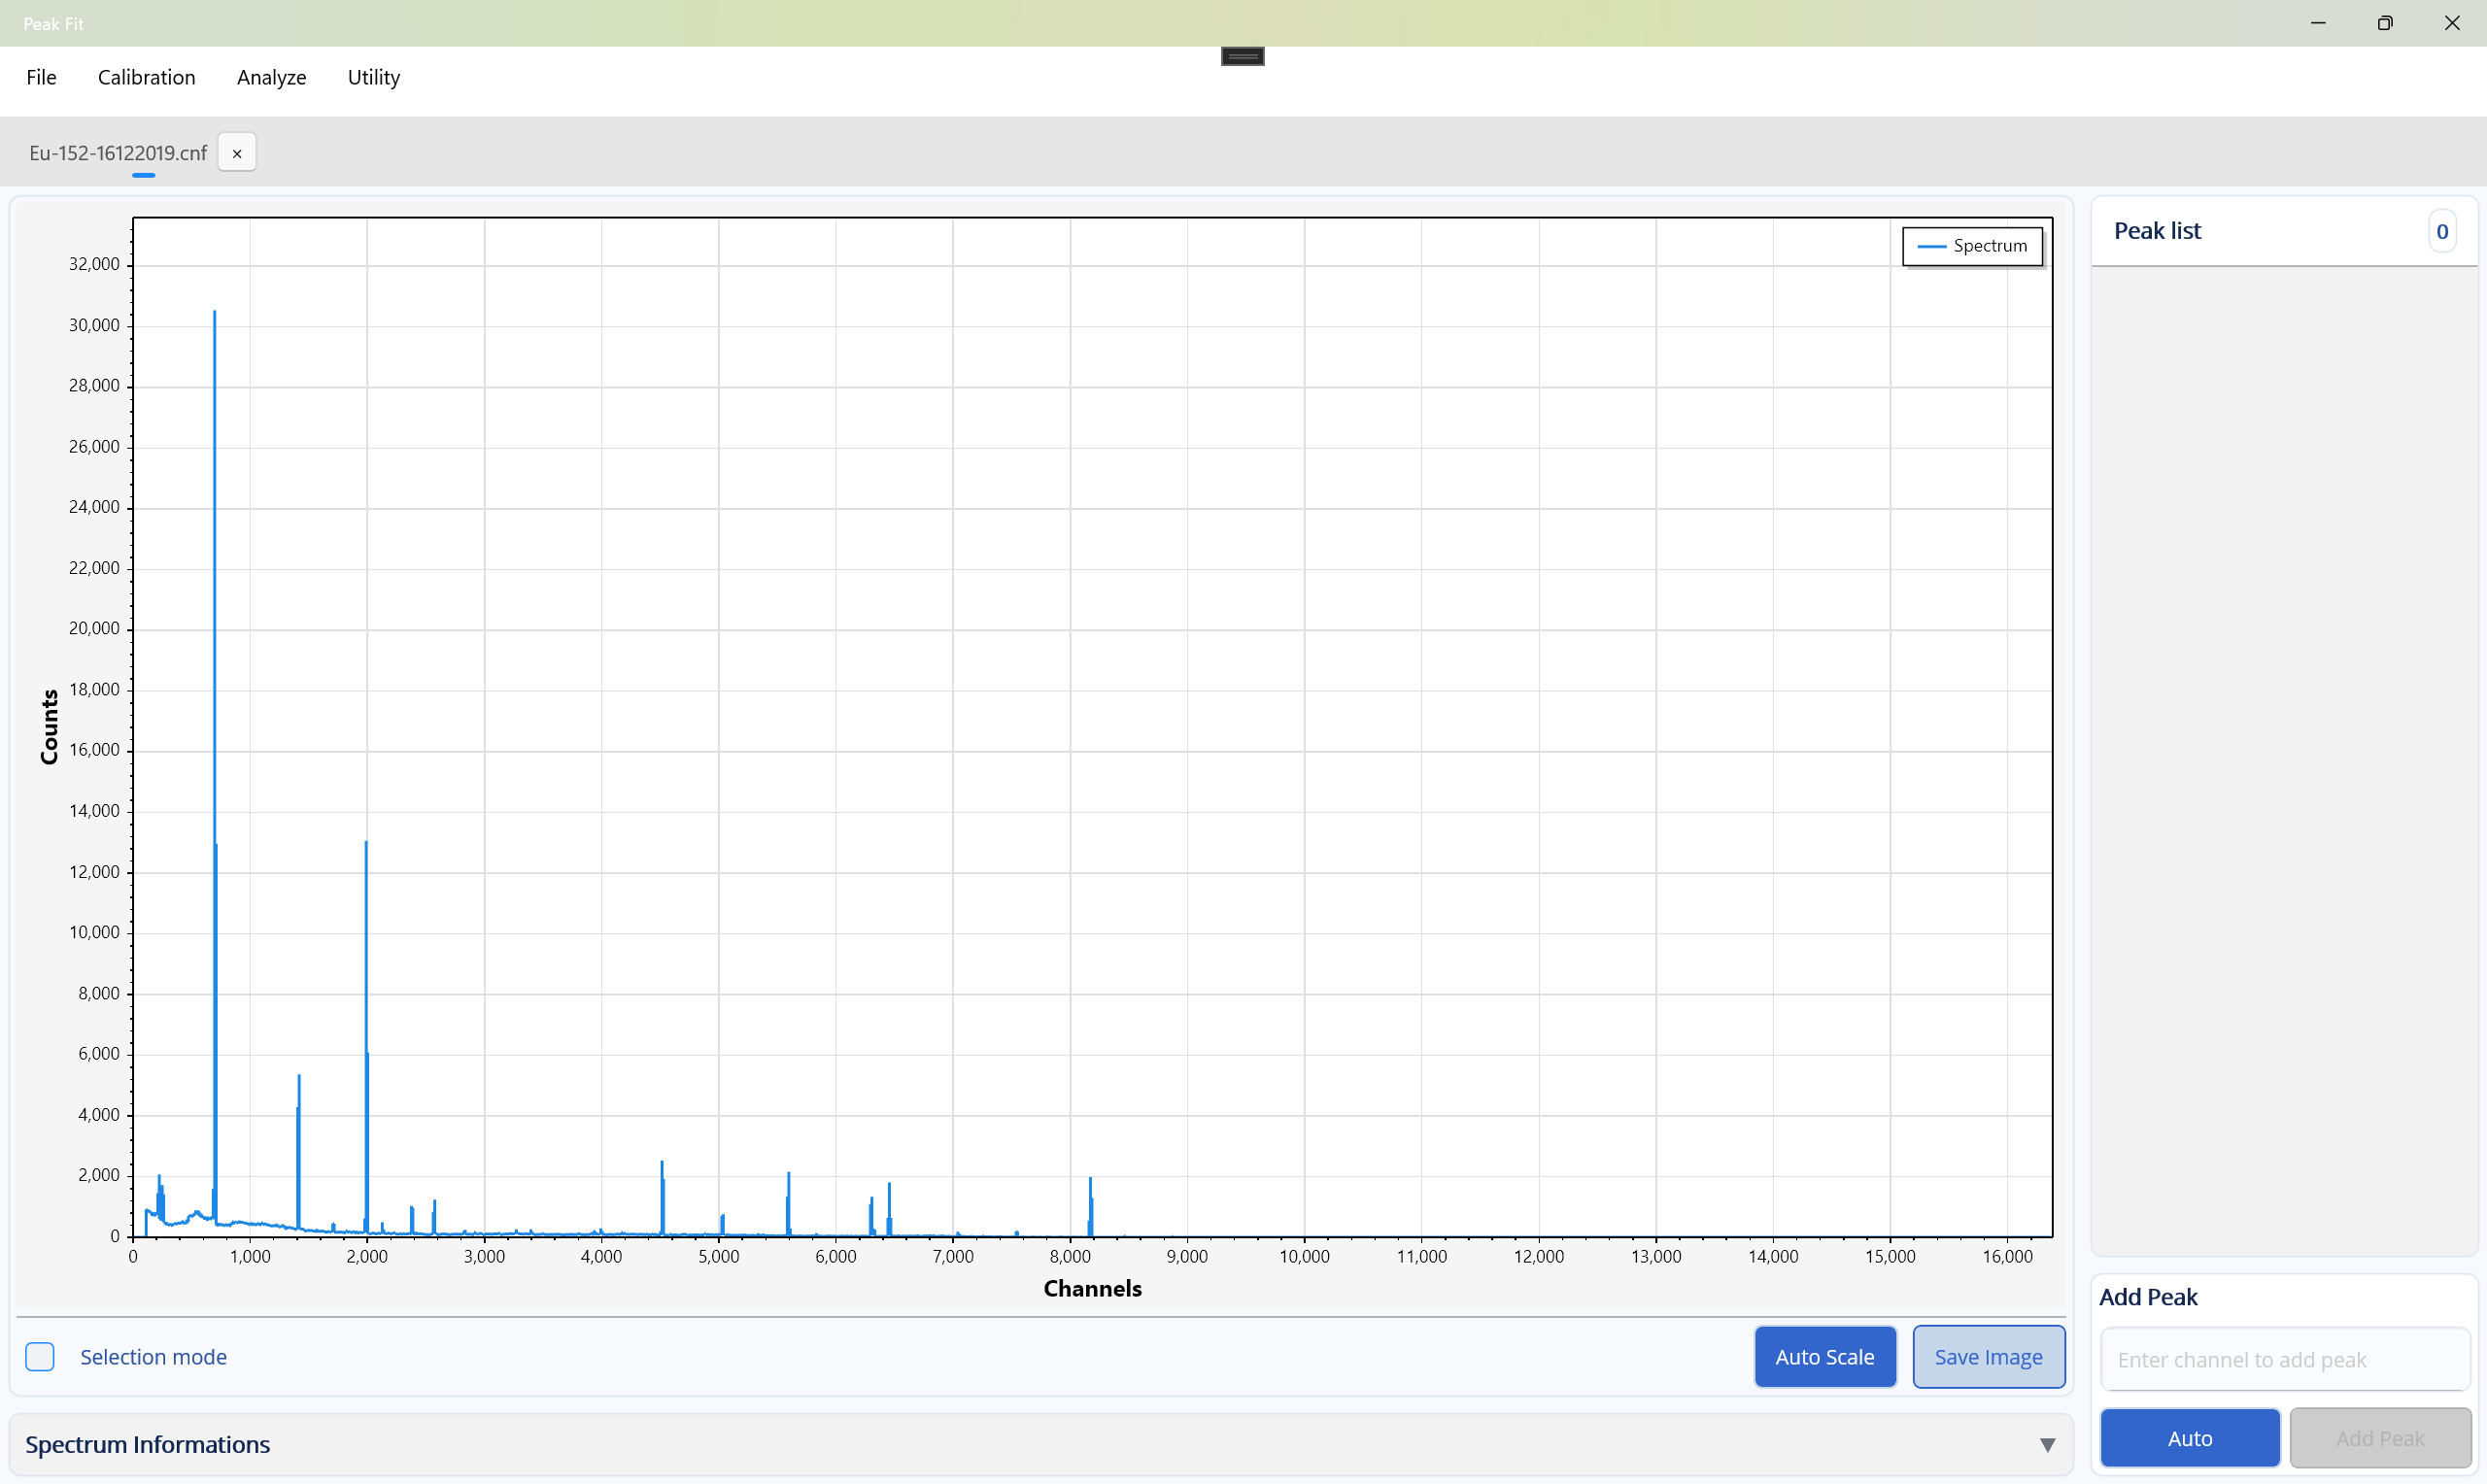
\includegraphics[width=0.8\textwidth]{img/spectrum.png}
						\caption{Phổ năng lượng của $^{22}\text{Na}$ và điểm đánh dấu đỉnh năng lượng bằng thuật toán}
						\end{figure}
					\item \textbf{ Hiệu chuẩn năng lượng và hiệu suất :}
						\begin{itemize}
							\item Hiệu chuẩn năng lượng :  thiết lập quan hệ giữa vị trí đỉnh năng lượng theo kênh và năng lượng gamma tham chiếu. Bằng phương pháp bình phương tối thiểu có thể xây dựng với đường chuẩn tuyến tính hoặc bậc hai : 
							\begin{equation}
								E(Ch) = \sum_{i = 0}^n a_i \cdot Ch^i
							\end{equation}
							\item  Hiệu chuẩn hiệu suất đầu dò : xây dựng đường cong hiệu suất theo năng lượng từ các điểm hiệu chuẩn. 	Bằng phương pháp bình phương tối thiểu có thể xây dựng với đường chuẩn hiệu suất đa thức bậc N: 
							\begin{equation}
								\ln(\epsilon) = \sum_{i = 0}^N a_i \cdot ln(E)^i
							\end{equation}
						\end{itemize}
					\item \textbf{Xác định độ rộng đỉnh (FWHM) : }\\
					\begin{itemize}
						\item Bước 1 – Xác định FWHM từng đỉnh: chọn các đỉnh từ danh sách ở mục 1, sau đó sử dụng thuật toán Levenberg-Marquardt để khớp dữ liệu  tại vùng đỉnh năng lượng với mô hình Gauss để xác định FWHM : 
						\begin{equation}
							y = A \exp\left(-\frac{(x-\mu)^2}{2\sigma^2}\right)
						\end{equation}
						\item Bước 2 – Xây dựng đường chuẩn FWHM: khớp các giá trị FWHM thu được theo năng lượng để ước tính độ rộng đỉnh trong dải đã hiệu chuẩn bằng phương pháp bình phương tối thiểu theo một trong các hàm sau : 
						\begin{gather}
							FWHM(E) = a \cdot \sqrt{E} + b\\
							FWHM(E) =  a\cdot E + b\\
							FWHM(E) = \sqrt{ a \cdot E + b } \\
							FWHM(E) = \sqrt{a\cdot E^2 + b \cdot E + c }
						\end{gather}
					
					\end{itemize}

				\end{enumerate} 
				

			\end{block}
			
		\end{column}
	
		\separatorcolumn
		
		\begin{column}{\colwidth}
			
			\begin{block}{Kết quả}
				Kết quả thu được từ phổ nguồn chuẩn $^{152}\text{Eu}$, $A = 26200\text{ Bq}$:

				\begin{figure}
					\centering
					\subfloat[]{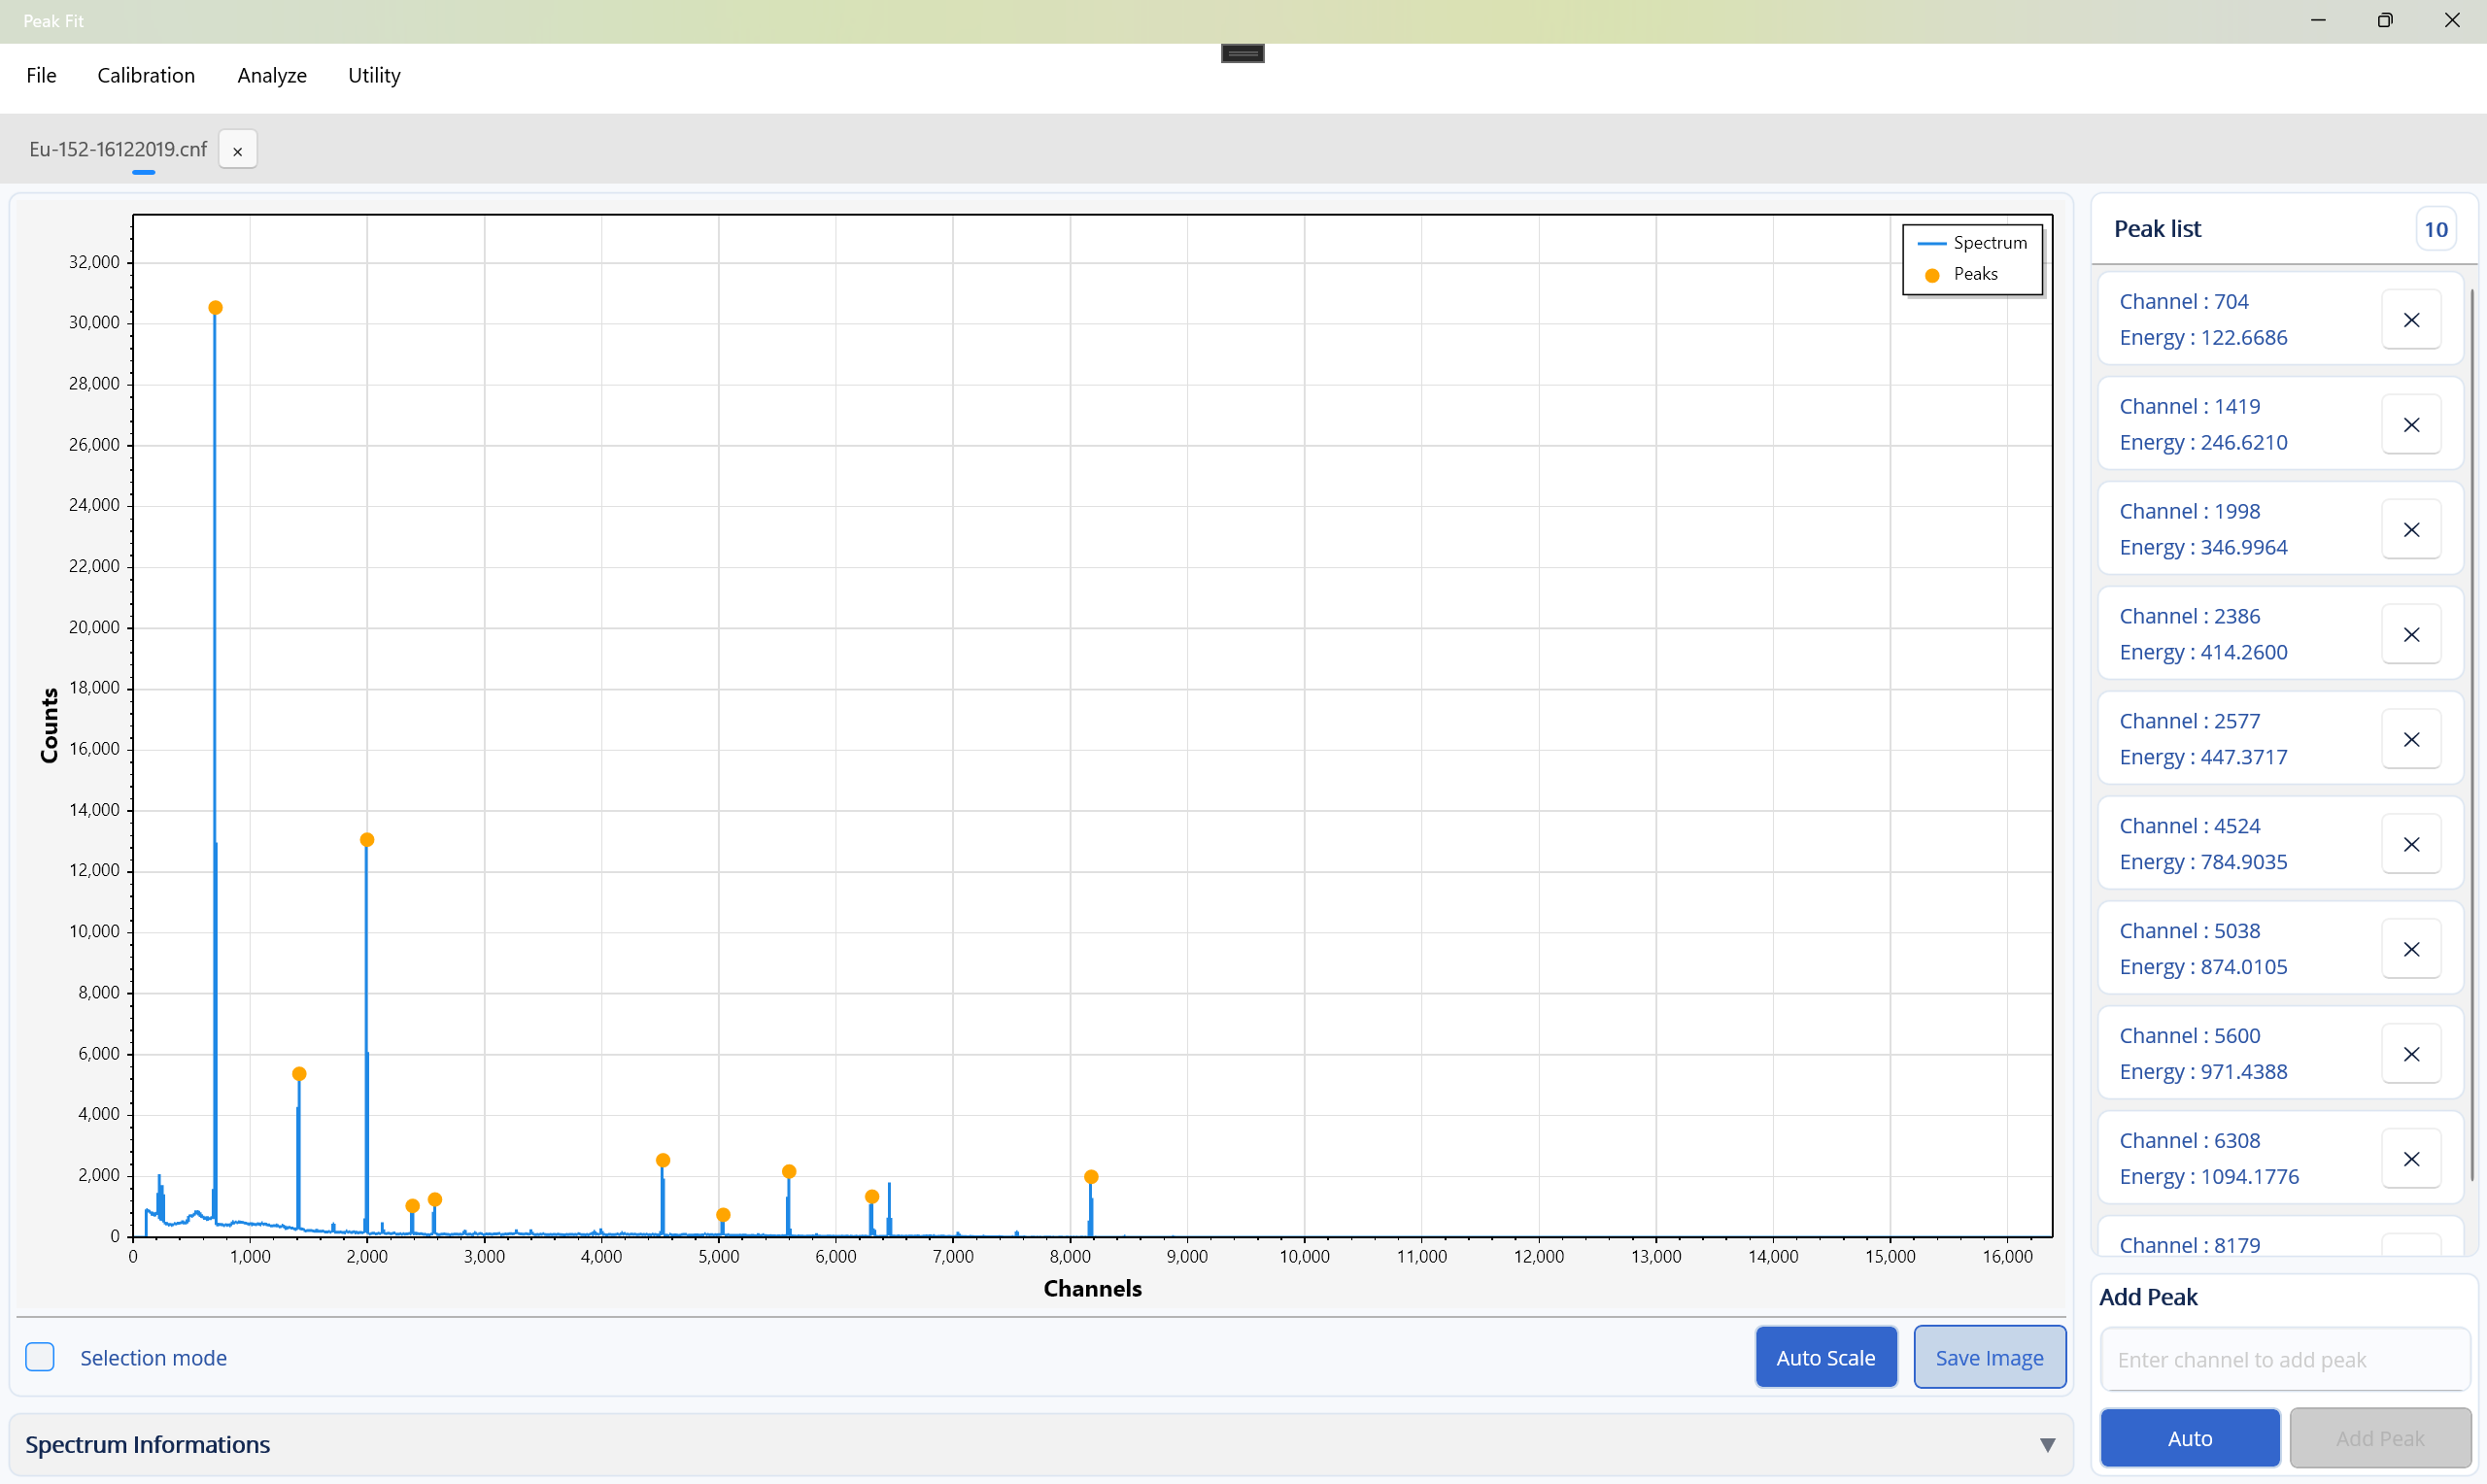
\includegraphics[width=0.48\textwidth]{img/Eu-152-16122019.png}}
					\subfloat[]{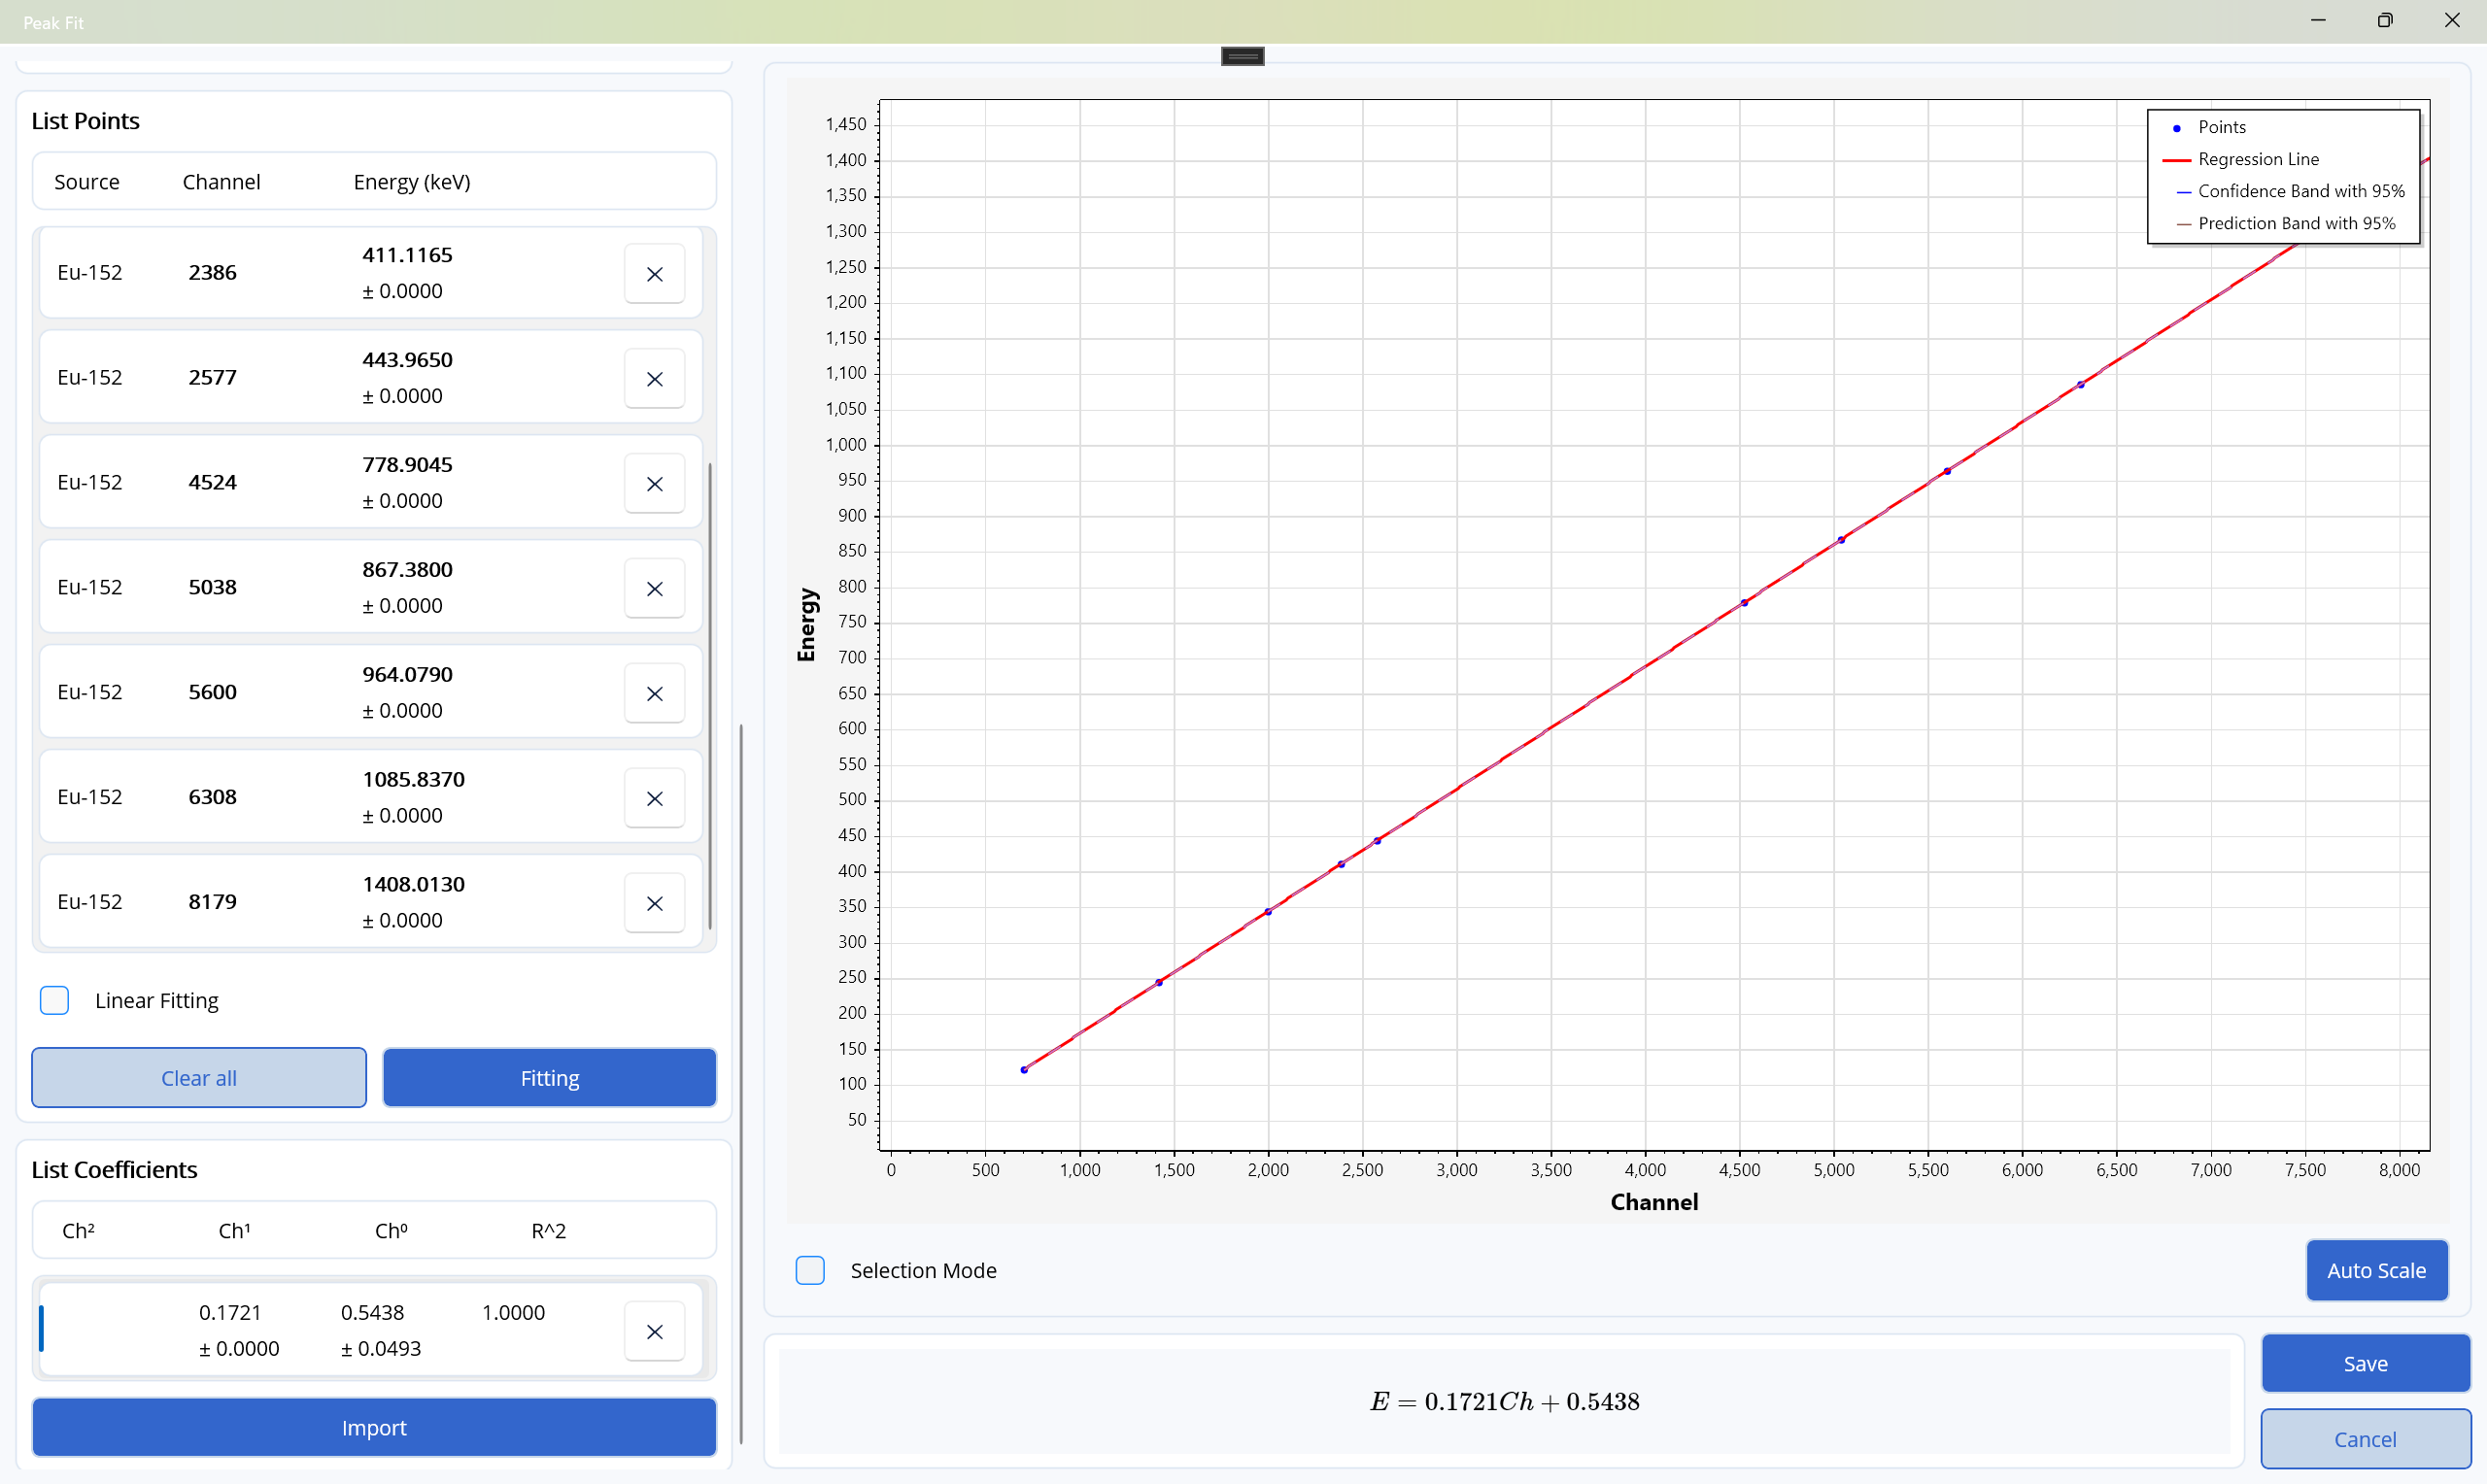
\includegraphics[width=0.48\textwidth]{img/Fit_E.png}} \\
					\subfloat[]{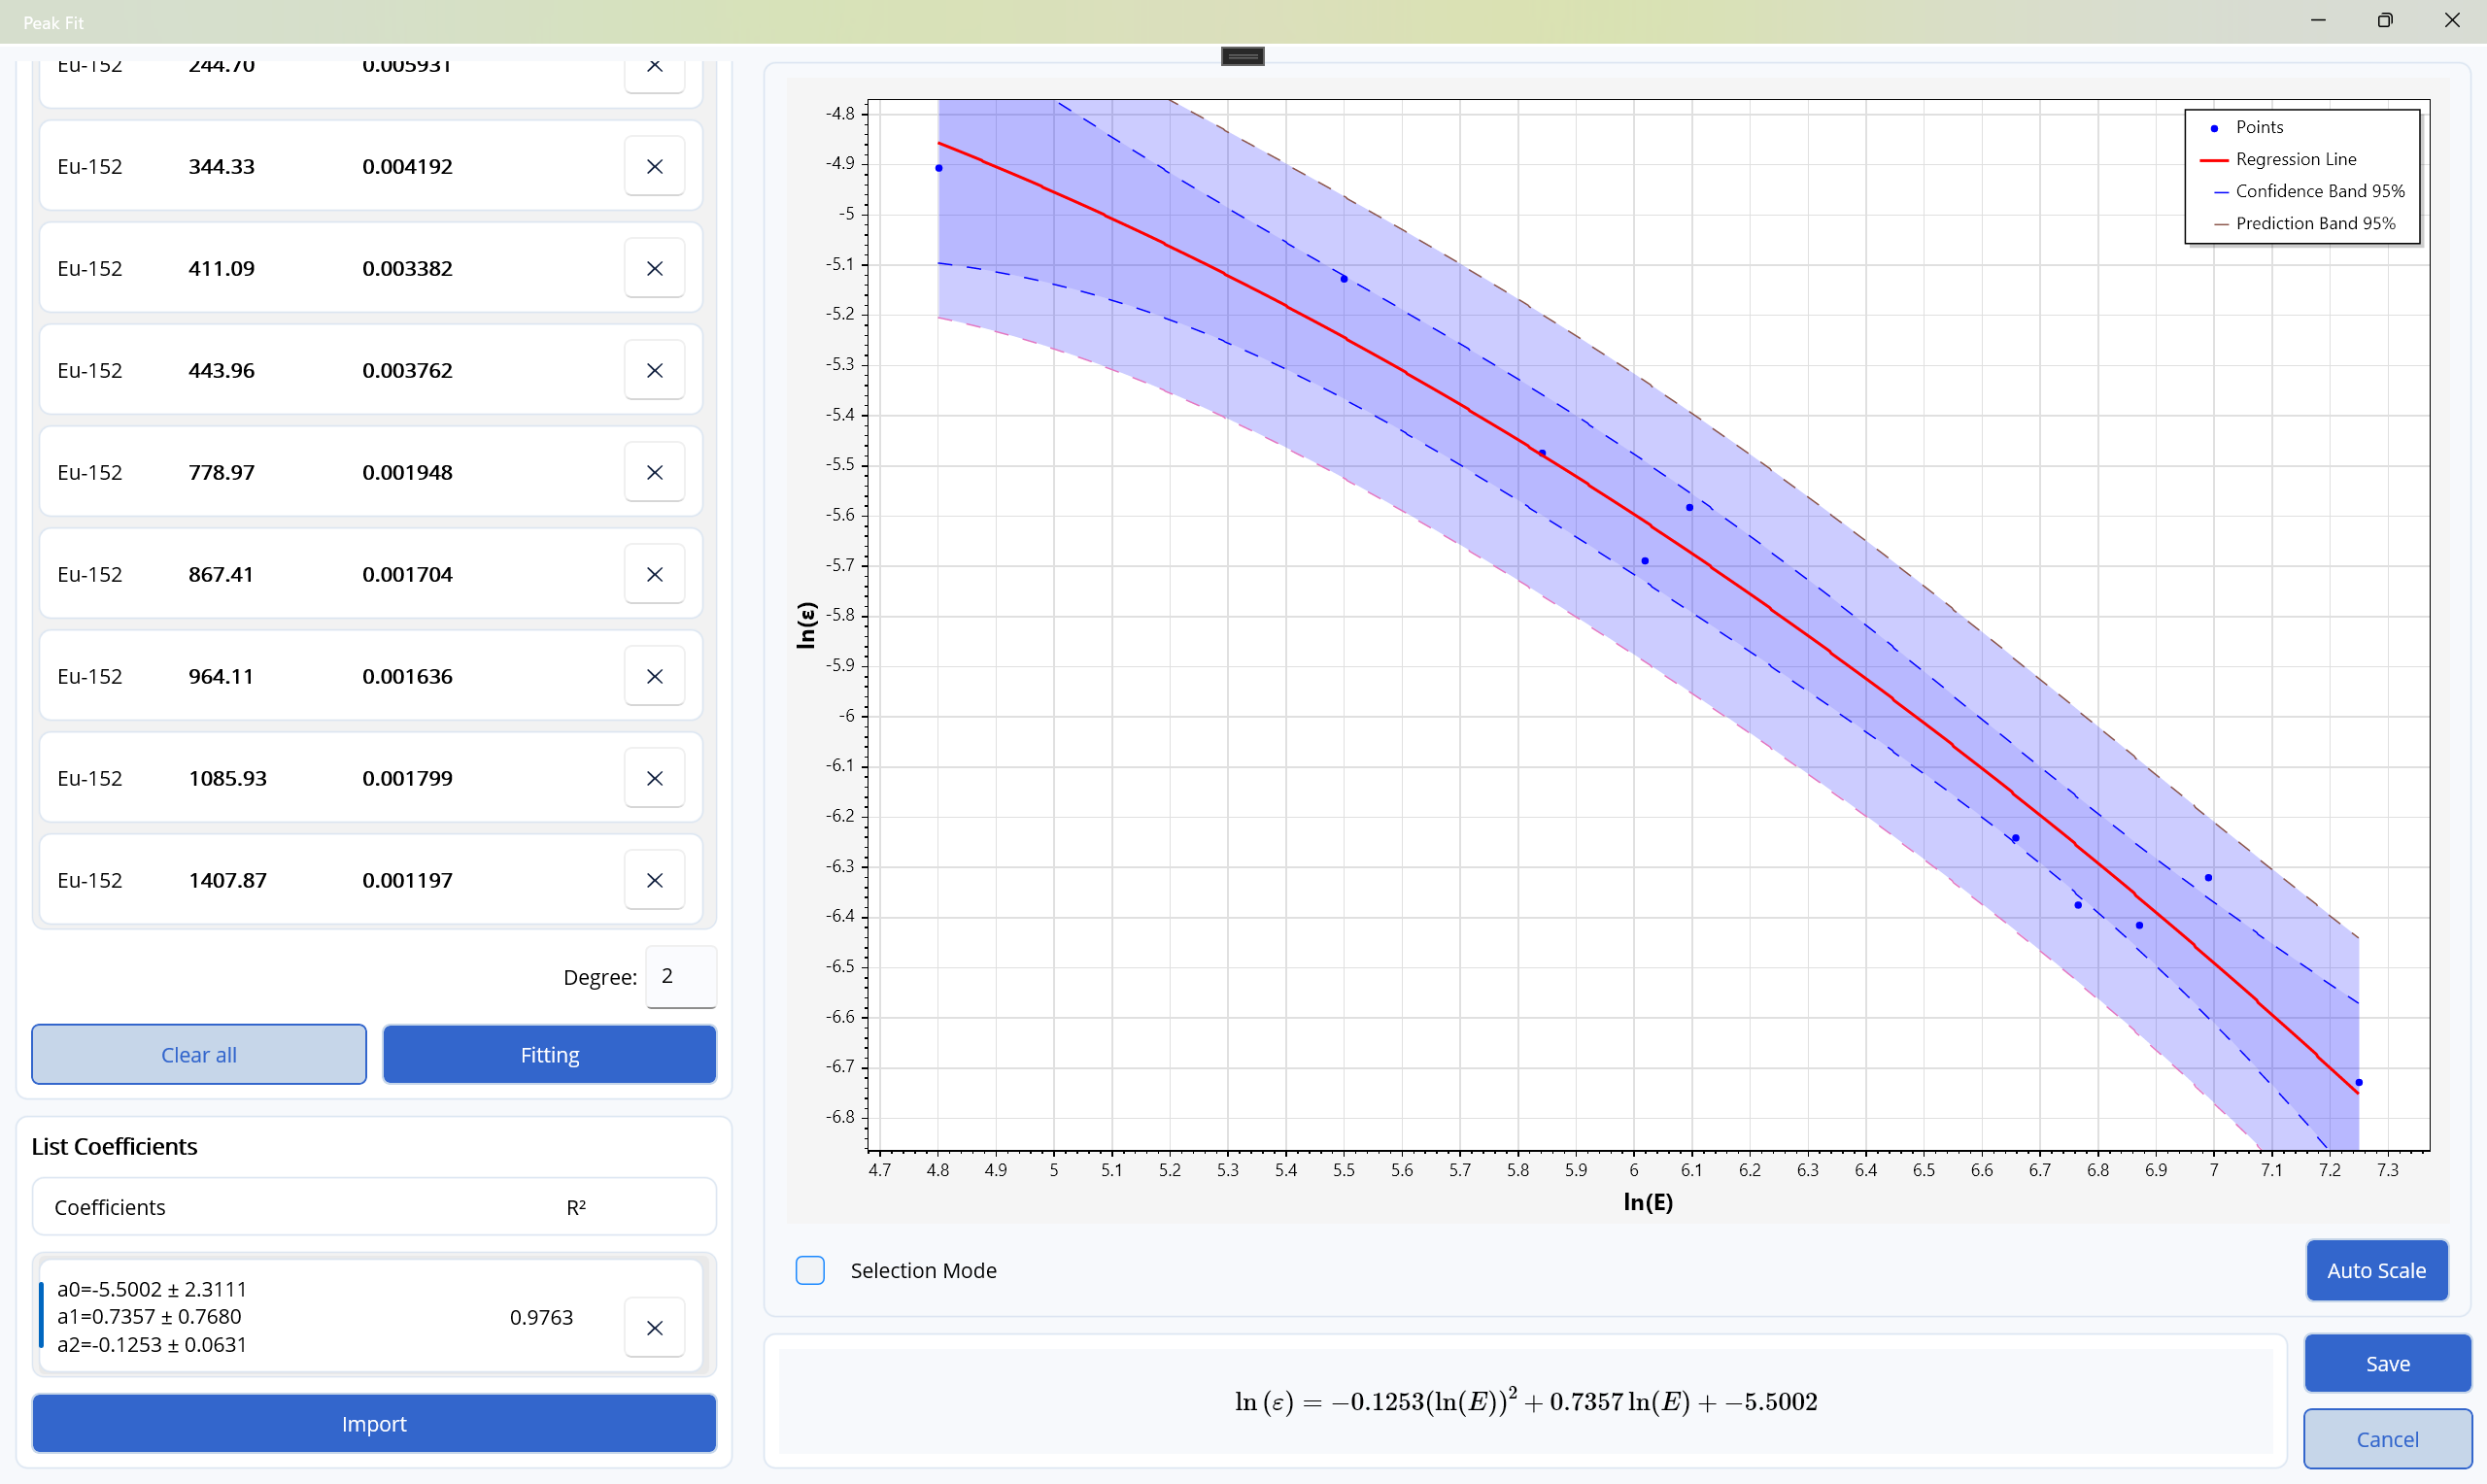
\includegraphics[width=0.48\textwidth]{img/Fit_eff.png}}
					\subfloat[]{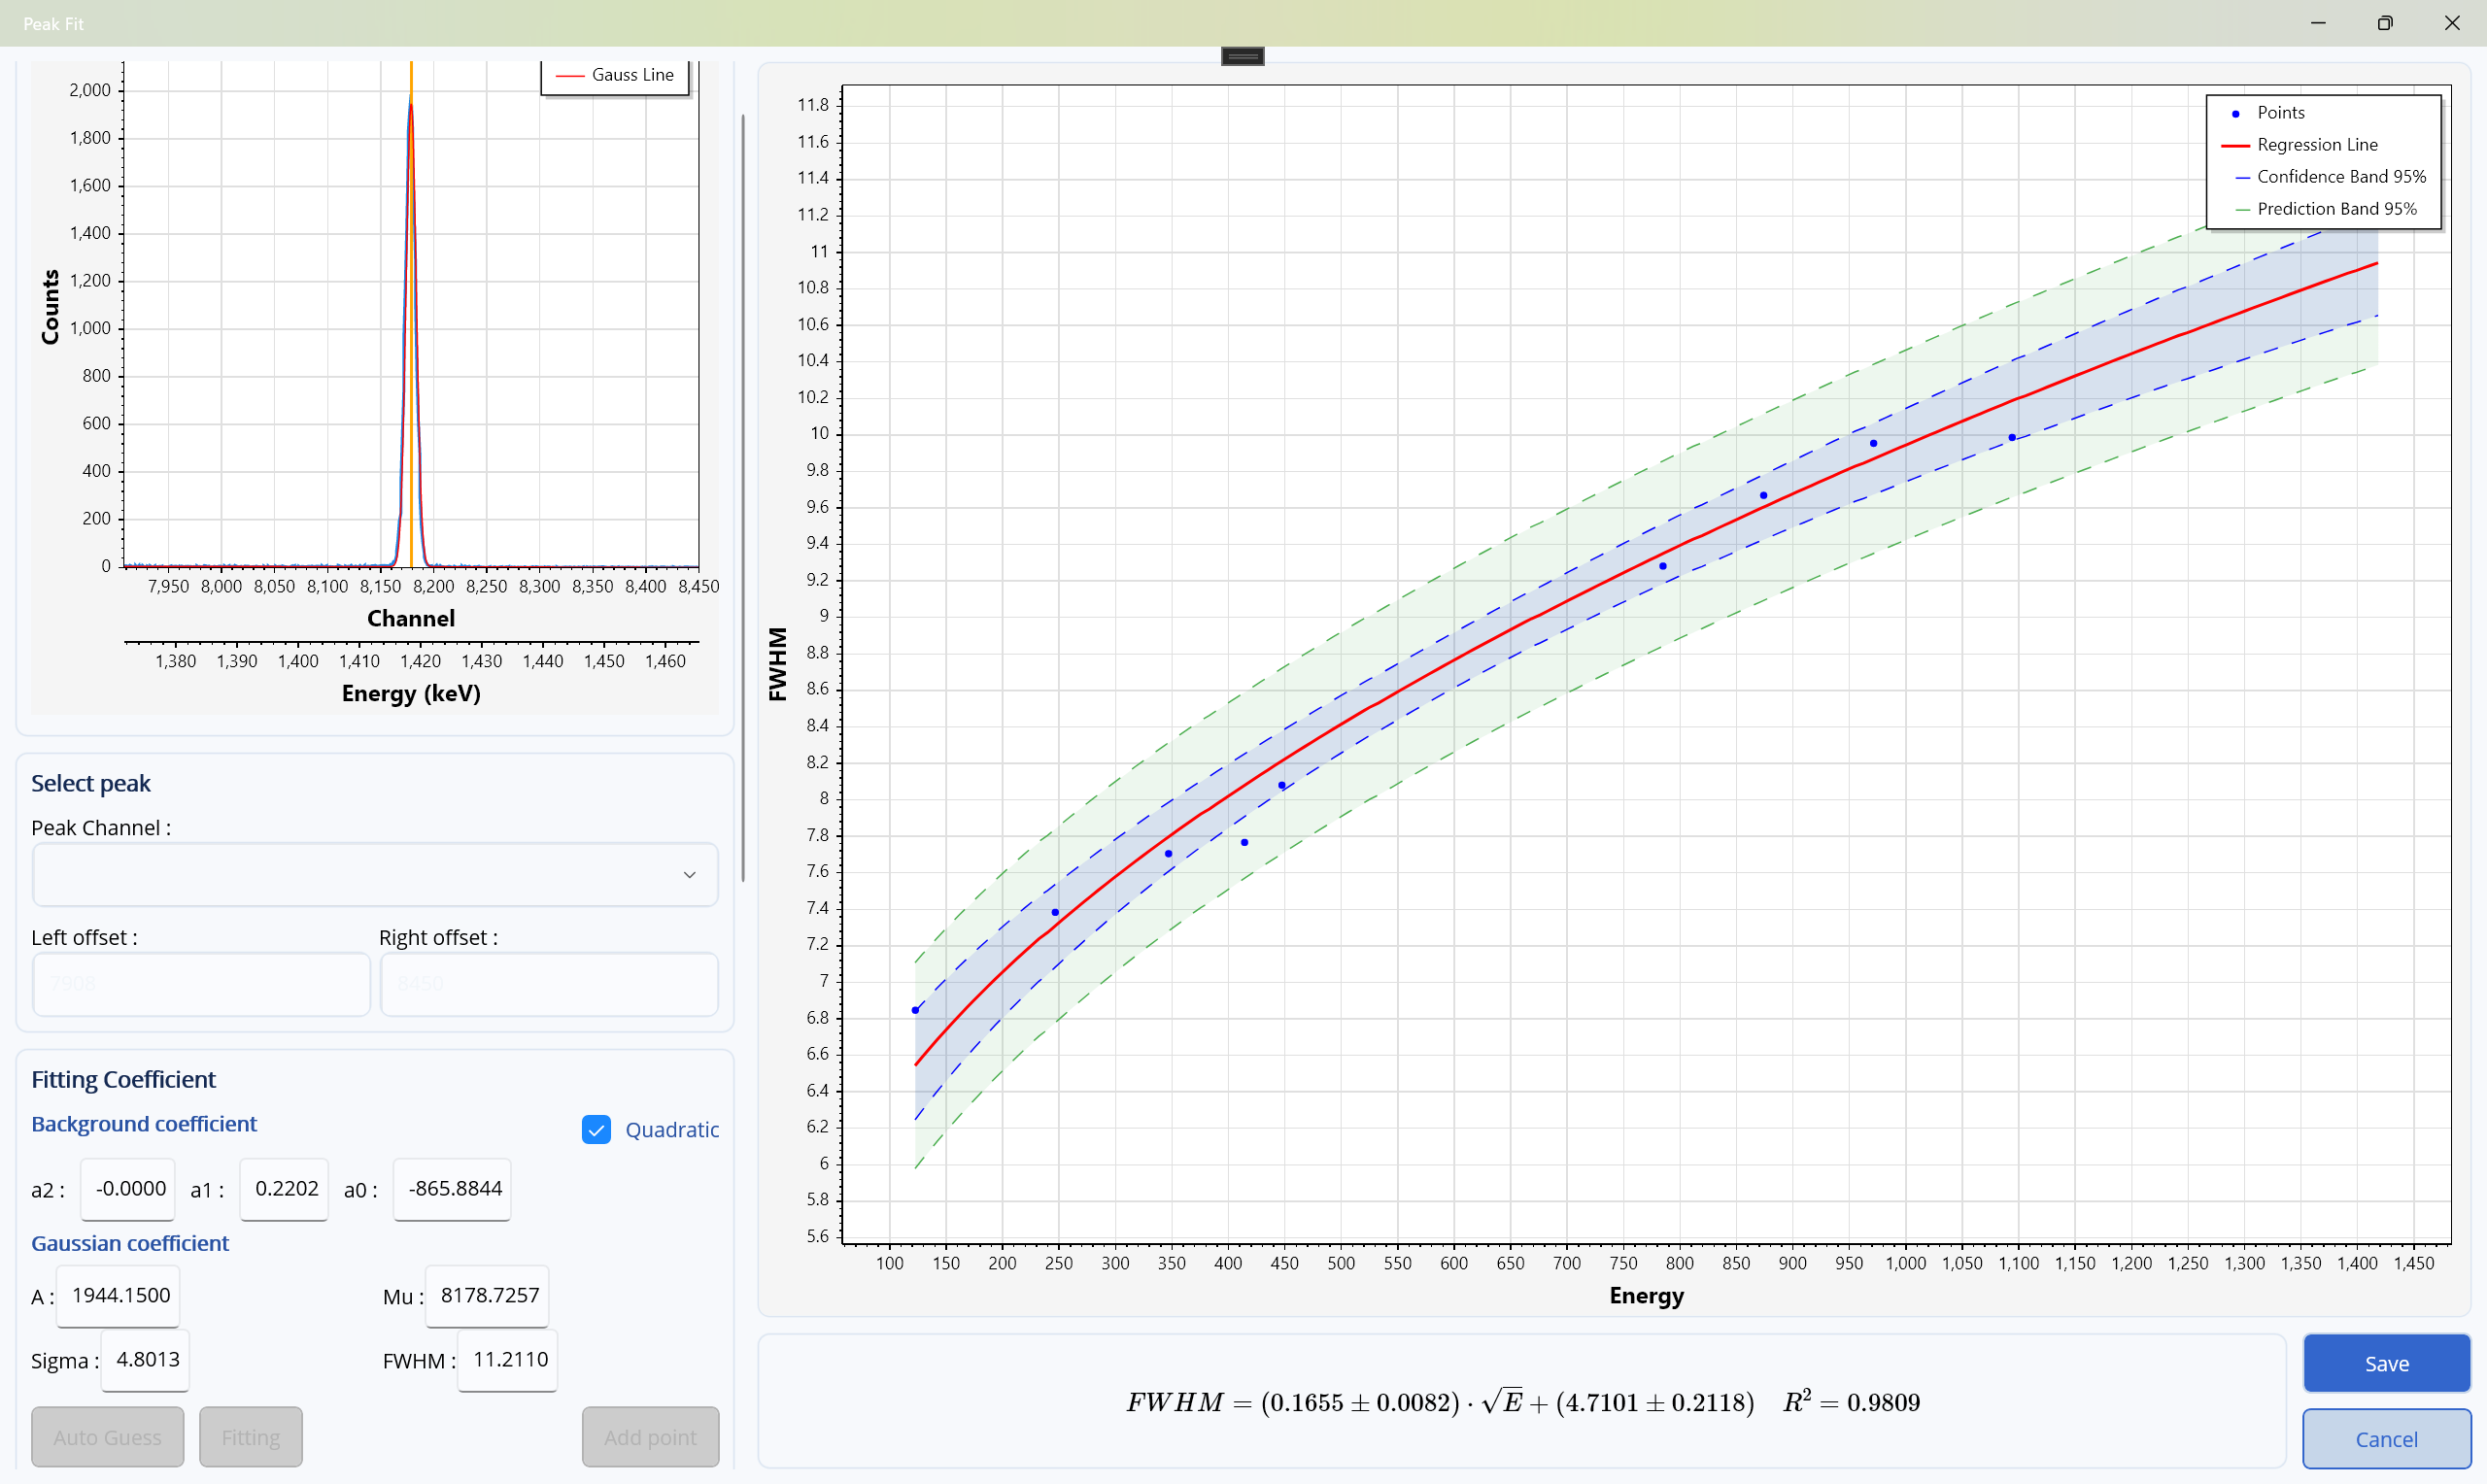
\includegraphics[width=0.48\textwidth]{img/Fit_FWHM.png}}
					\caption{(a) Phổ $^{152}Eu$ với các điểm đánh dấu vị trí đỉnh năng lượng 
					 (b) Đường chuẩn năng lượng 
					 (c) Đường chuẩn hiệu suất 
					 (d) Đường chuẩn bề rộng một nửa (FWHM)}
				\end{figure}
				\begin{enumerate}
					\item Nhận diện đỉnh tự động : \\
					Số đỉnh tìm được 10/14 đỉnh (đỉnh có cường độ trên 1\%), với tham số ban đầu là : 
					\begin{itemize}
						\item $w = 5$ 
						\item $\epsilon = 10$
						\item $f = 20$
					\end{itemize}
					\item Phương trình đường chuẩn năng lượng:
					 \begin{equation}
						E = (0,1721 \pm 0,0000)\cdot Ch + (0,5438 \pm 0,0493) \, (KeV)
					\end{equation}
					$R^2 = 1$
					\item Phương trình đường chuẩn hiệu suất :
					 \begin{equation}
						\ln(\epsilon) = (-0,1253 \pm 0,0631) \cdot \ln(E)^2 + (0,7357 \pm 0,7680) \cdot \ln(E) + (-5,5002 \pm 2,3111)
					\end{equation}
					$R^2 = 0,9763$
					\item Phương trình đường chuẩn bề rộng một nửa (FWHM) : 
					\begin{equation}
						FWHM = (0,1713 \pm 0,0078)\cdot \sqrt{E} + (4,6226 \pm 0,2010)
					\end{equation}
					$R^2 = 0,9808$
				\end{enumerate}
			\end{block}
			
			\begin{block}{Kết luận}
			\begin{itemize}
				\item Đã sơ bộ xây dựng thành công phần mềm PEAKFIT ứng dụng trong phân tích phổ tia gamma.
				\item Phần mềm tự động hóa quy trình nhận diện đỉnh thông qua thuật toán Mariscotti, đồng thời tích hợp thành công các công cụ hiệu chuẩn năng lượng, hiệu chuẩn bề rộng một nửa (FWHM) và hiệu chuẩn hiệu suất. Với chuẩn bề rộng một nửa phần mềm xử lý tính toán tốt các tham số ban đầu theo thuật toán Levenberg-Marquardt và kết quả FWHM.
				\item Kết quả thử nghiệm trên phổ thực nghiệm cho thấy sự ổn định của phần mềm, với khả năng nhận diện tự động {\bf 10/14} đỉnh phổ (các đỉnh có cường độ lớn hơn 1\%) và thiết lập các đường chuẩn thực nghiệm có độ chính xác cao.
			\end{itemize}	
			\end{block}
			
			
			\begin{block}{Tài liệu tham khảo}
				\printbibliography[heading=none]
			\end{block}
		\end{column}
		
		\separatorcolumn
	\end{columns}
\end{frame}
\end{document}